\section{Results}
\label{sec:results}
\subsection{Traditional approaches fail to adequately remove batch effects when covariate overlap is poor}
\label{sec:results:sims}
We constructed simulations to help us understand the differences between associational or conditional reasoning and causal reasoning. To this end, we evaluate the performance of our proposed technique, \cccombat, in comparison with two conditional approaches one may use for batch effect correction, including \ccombat~\cite{Johnson2007Jan} and \combatgam~\cite{Pomponio2020Mar}, which leveraged generalized additive models (GAMs) to capture non-linear trends related to age.

Figure \ref{fig:sim_nlin_adjust}(A).I. shows a simulation where the outcome of interest (e.g., a feature of a connectome, $y$-axis) is associated with a covariate of interest ($x$-axis) through a non-linear relationship (the sigmoid). If samples are from the blue batch, they are offset $1$-unit higher than samples from the orange batch. $N=500$ samples are drawn with equal probability from each batch. In the high overlap regime, the orange and blue batches have the same covariate distribution. Figure \ref{fig:sim_nlin_adjust}(B).I. shows the expected signal (solid line) for each batch, along with the difference between the expected signal for each batch (gray box). These curves are shown along with the group-specific linear model fit (dashed lines) estimated from the sample points, which is the model that is later used by \ccombat~for batch effect adjustment. Figure \ref{fig:sim_nlin_adjust}(C).I. and Figure \ref{fig:sim_nlin_adjust}(D).I. show the impact that \ccombat~and \cccombat~have on the expected signal at a given covariate level. Intuitively, one would anticipate that a batch effect correction strategy should place the expected signals virtually overlapping after correction, since the batch effect is characterized by the expected signals in each group differing by an offset factor. For both strategies, the expected signal after correction is virtually the same for each of the two batches, indicating that the batch effect has been successfully removed. \edits{We compute the mean average absolute difference (AAD) across included covariate values of the two lines over $R=1$,$000$ trials, where a mean AAD of $1$ corresponds to the residual disparity on average equaling the original batch effect, and a mean AAD of $0$ corresponds to no residual disparity. The mean AAD is discussed in Appendix \ref{app:maad}. We find that \ccombat~has a mean AAD of $.058$, and \cccombat~a  mean AAD of $.047$, with \cccombat~having a lower mean AAD about $62\%$ of the time.}

Figure \ref{fig:sim_nlin_adjust}(A).II. shows similar plots; however, the covariate distributions have been shifted such that they no longer overlap perfectly. The orange batch has a left-shifted covariate distribution, and the blue batch has a right-shifted covariate distribution (the covariate is \textit{confounding} the relationship between the outcome and the batch). Figure \ref{fig:sim_nlin_adjust}(B).II. shows that while the expected signal in each batch at a given covariate level is the same as in Figure \ref{fig:sim_nlin_adjust}(B).II., the linear model fits for each group estimated from the sample now differ (the lines are rotated slightly in a clockwise direction, and are now offset further apart). Figure \ref{fig:sim_nlin_adjust}(C).II. shows that after correction, the expected signal at each covariate level do not overlap; in fact, they differ more after correction than before. This is because the model being employed by \ccombat~is biased under the given true data distribution. Figure \ref{fig:sim_nlin_adjust}(D).II. shows that, unlike \ccombat, \cccombat~restricts inference to the region of shared covariate overlap between the two batches, and does not perform inference that is unsupported by the data. This is indicated by the fact that the expected signal after correction has been restricted to no longer include the left-most and right-most portions of the covariates. Within this region, the expected signal for each batch after correction are much closer, indicating that the batch effect has been nearly entirely removed after \cccombat. \edits{Over all trials, we find that \ccombat~has a mean AAD of $1.04$, and \cccombat~a mean AAD of $0.22$, with \cccombat~always having a lower mean AAD.}

Figure \ref{fig:sim_nlin_adjust}(A).III. has furthered this trend such that there are almost no samples in a region of shared covariate overlap between the two batches. In Figure \ref{fig:sim_nlin_adjust}(B).III. the expected signal in each batch at a given covariate level is the same as in Figure \ref{fig:sim_nlin_adjust}(B).I., but the per-group linear model fits are now even further offset. \edits{This has the effect that in Figure \ref{fig:sim_nlin_adjust}(C).III., the expected signal after correction has a mean AAD of $3.03$, exceeding the original batch effect by over $200\%$.} On the other hand, \ref{fig:sim_nlin_adjust}(D).III. shows that \cccombat~would indicate to not perform inference at all on the batches due to the fact that there are no portions of the covariate range in which the two batches have samples which could be compared. \edits{\cccombat~only executes on $26$ of the trials, and has a mean AAD of $0.369$, always lower than that of \ccombat~for trials in which it could be executed.}

\begin{figure}[h]
    \centering
    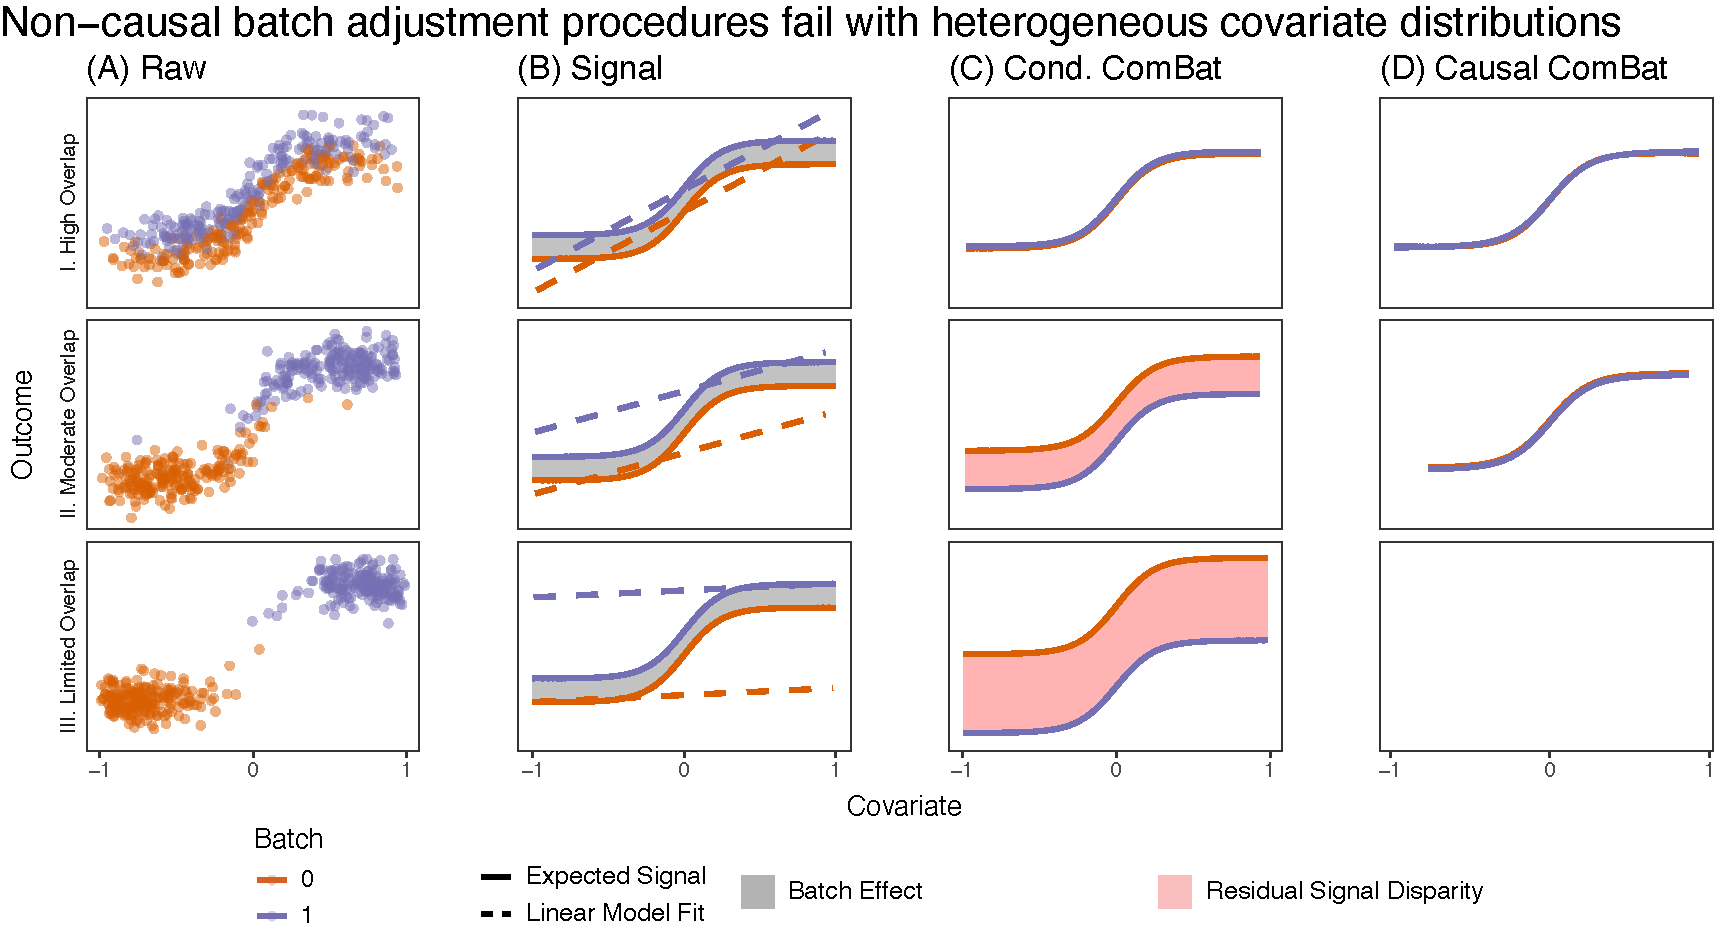
\includegraphics[width=\linewidth]{Figures/Content/sim_nlin_adjust.pdf}
    \caption{\textbf{Non-causal procedures are subject to strong biases without covariate matching}. $N=400$ points are simulated from either batch $0$ or batch $1$ in (A). In (B), the expected signal at a given covariate level is indicated by the solid lines. The batch effect is the difference between the two solid lines (gray box). The estimated linear model fit employed by \ccombat~is indicated with the dashed line. After adjustment (C. and D.), the original expected signal relationship is passed through the trained model, and any residual difference between the true signals of the two batches is termed a residual signal disparity (red box). When coverlap overlap is high in I, both \ccombat~and \cccombat~remove the batch effect successfully, and the expected signal after correction accurately overlaps. With moderate covariate overlap in II, the limitations of the \ccombat~model introduce residual bias that results in an over-correction of the batch effect (on average, the residual signal difference is about about equal to the original batch effect). While \cccombat~reduces the covariate space for inference to remove samples with covariates unlike the other batch (the covariate region to the far left and far right), the samples within the region of covariate overlap are in general reasonably corrected for a batch effect without corrupting the covariate/outcome signal relationship (on average, the residual signal difference is about $20\%$ the original batch effect). When covariate overlap is low in III, Causal strategies tend to report that no inference can be performed, which in our opinion, is the correct procedure. On the other hand, conditional strategies may impart substantial residual signal disparities (on average, about $300\%$ the scale of the original batch effect).}
    \label{fig:sim_nlin_adjust}
\end{figure}

In Appendix \ref{app:sim_effect} and Appendix \ref{app:sim_batch_adj}, we explore further implications of using causal techniques for batch effect detection and removal (and more broadly, causal effects in general) respectively across both linear and non-monotonic regimes to supplement the non-linear regime investigated here. Conceptually, researchers may feel as though they are left with a tradeoff:
\begin{enumerate}[leftmargin=*]
    \item When datasets do not have high overlap demographically, the (implied or explicit) limitations of a model leveraged by a batch effect detection or correction technique can impart substantial bias on the conclusions of the investigation. While the limitations or shortcomings may \textit{seem} inconsequential, the scale of the residual signal disparities imparted can dwarf the original batch effect, and yield measurements which are \textit{more} dissimilar than prior to batch effect adjustment, as we saw in Figure \ref{fig:sim_nlin_adjust}(C).II. and (C).III.
    \item Enforcing demographic overlap mechanistically through propensity trimming and/or matching may \textit{seem} like it yields fewer samples for analysis, or narrows the scope of conclusions.
\end{enumerate}
In practice, the reality is that with biological data, there are \textit{no} ground truths. As a result, there is no way to evaluate the introduction of imparted residual bias, and no way to know whether downstream conclusions are a product of imparted residual biases. This means that any statistical inference we derive may be arbitrarily true or false, and we have no way of qualifying in which pool our inference stands. 

When we mechanistically re-weight the data to impose demographic overlap, proper statistical inference tempers conclusions as a direct consequence of the smaller demographic region under consideration. Stated another way, this means that when we balance \textit{prior to} detecting or correcting for batch effects, we have tools which allow us to make internally valid conclusions supported by the data in regions in which the data \textit{are able}. This means that, although our conclusions may not apply to the \textit{entire} region of covariate support in the observed data (such as, in Figure \ref{fig:sim_nlin_adjust}(D).II., where we were only able to perform analysis in the region of shared support), they will be \textit{statistically and methodologically valid} with respect to the re-weighted population that we \textit{did} analyze.

\subsection{Detecting Batch Effects in the CoRR mega-study}

\begin{figure}[h]
    \centering
    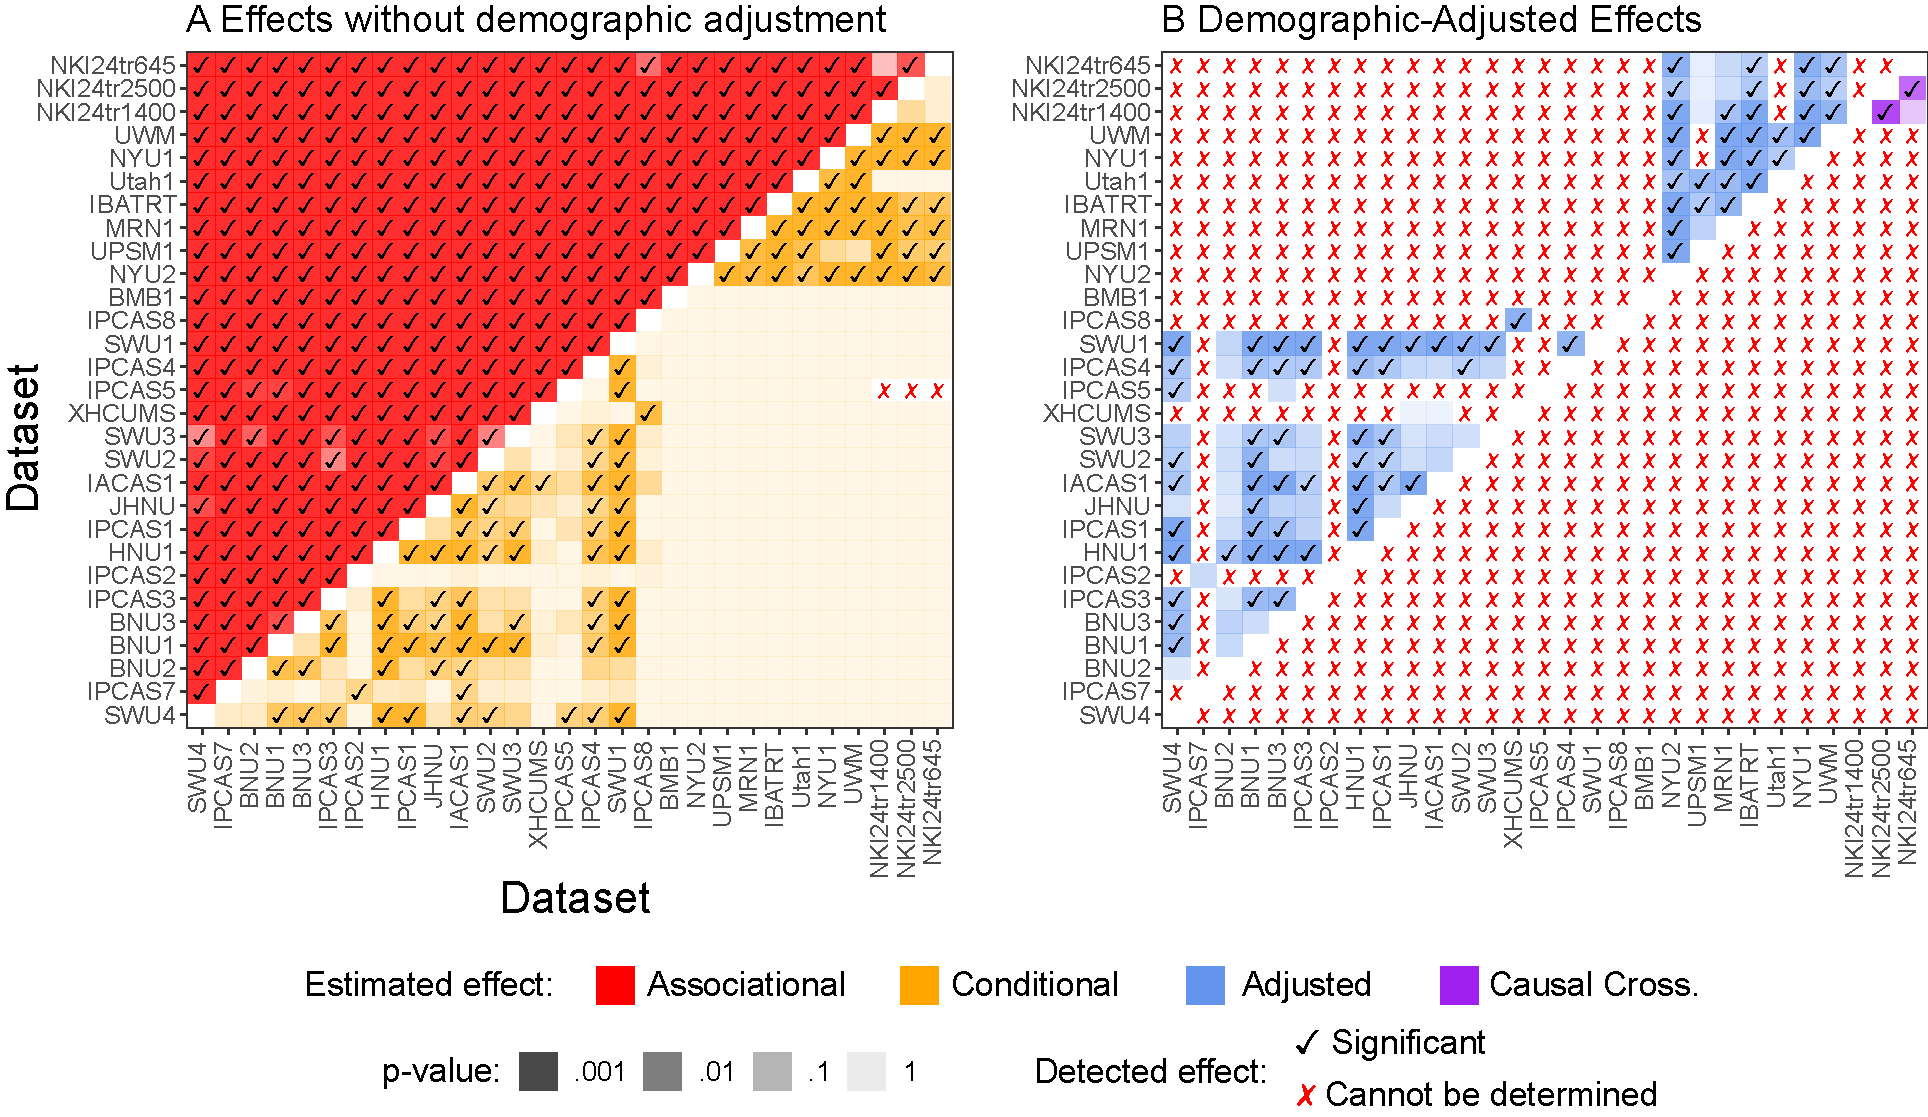
\includegraphics[width=\linewidth]{Figures/Content/raw_pairwise.pdf}
    \caption{\textbf{Comparison of Estimated Effects for CoRR Mega-Study}. Heatmaps indicating the $p$-value of effect estimates per pair of studies. Studies are organized by continent, followed by the number of samples in the study. Comparisons which are significant at $\alpha=.05$ are indicated by a black check. Since effects are symmetric (an effect between batch $t$ and $t'$ is equivalent to an effect between batch $t'$ and $t$), we collapse symmetric heatmaps into a single triangle for each effect type. \textbf{(A)} Effects which can be estimated but do not make direct adjustments for demographics. Associational and conditional effects can almost always be estimated between pairs of studies, so long as they share overlap in at least one covariate (IPCAS5 and NKI24 studies are entirely male or entirely female, entirely different continents, and entirely different age distributions, respectively, red Xs). \textbf{(B)} Effects which adjust for demographics through covariate adjustment. Squares in which an effect was not estimable due to covariate misalignment are indicated by a red X. Effects which adjust for demographics require covariate overlap across all covariates, which is indicated in Figure \ref{fig:demographic}B. A direct comparison of Figure \ref{fig:demographic}B between the conditional and adjusted procedures reveal that whereas conditional procedures tend to ``fail to reject'' with low or zero covariate overlap, adjusted procedures tend to avoid inference entirely.
    }
    \label{fig:raw_pairwise}
\end{figure}

Figure \ref{fig:raw_pairwise}A explores the four effects defined above in fMRI connectomes from the CoRR mega-study. {\edits{The majority of associational effects (99.8$\%$) are significant (distance correlation two-sample test, BH correction, $\alpha=0.05$). When we account for demographic covariates using conditional approaches, this drops to 25.8\% (conditional distance correlation two-sample test, BH correction, $\alpha=0.05$). Conceptually, both of these approaches are overly simplistic for concluding that a causal batch effect is indeed present because they fail to account for non-overlap of the covariate distributions between the subjects. In statistics, this is known as a ``fail to reject''; statistical inference via the conditional approach simply indicates to us that there is no evidence to reject the null hypothesis, and does not provide evidence for the null hypothesis (there is no effect). However, many of these comparisons are simply unreasonable to make in the first place.}}

Effects that account for demographic distributions are examined in Figure \ref{fig:raw_pairwise}B. Many pairs of studies could not have an adjusted effect estimated due to poor demographic alignment as shown in Figure \ref{fig:demographic}B, which resulted in no suitable matches existing between the studies, indicated by a red X ($279$ of $406$ pairs of studies). \textcolor{black}{Colloquially, when covariate overlap is moderate or limited as in Figure \ref{fig:sim_nlin_adjust}, we cannot tell if effects are misrepresented (or, comparisons are unreasonable entirely) due to demographic imbalance. In this way, causal strategies pre-pended to batch effect detection and mitigation strategies are \textit{more conservative in their application}, in that they prevent the experimenter from potentially deriving spurious or erroneous conclusions due to confounding biases, and directly indicate when comparisons are unreasonable to make}. Notably, adjusted conditional effects are estimable between all pairs of the American Clique (a group of separate studies consisting of similar demographics collected in North America, consisting of NYU1, NYU2, IBATRT, UWM, MRN1). After adjustment for the sample characteristics of the demographics associated with individual studies, a majority of adjusted effects (67.8$\%$) remain significant (causal conditional distance correlation two-sample test, BH correction, $\alpha=0.05$). 

The NKI Rockland Sample takes this a step further, allowing a crossover effect to be determined in a few pairs of batches (purple squares). This study was, in fact, collected on an identical set of participants, in the same location, with the same research technicians, with data varying only in the repetition time for the magnet used in the scanner. Indeed, for two of three comparisons, crossover effects remain prominent. This provides evidence that the parameters under which a study are conducted is a causal predictor of measured connectomes, assuming no participant state confounders are present.

% Word site effect => effect, but be clear we mean the effects discussed in 2.1
\label{sec:study_est_adjustment}

\subsection{Traditional Approaches Produce Disparate Inference from Techniques which Leverage Causality}
\textcolor{black}{At this point, we have demonstrated, through simulation and real examples, if a covariate is a \textit{confounder}, failure to properly account for demographic balancing can, potentially, yield improper detection and mitigation of batch effects and may, in turn, fundamentally alter true signals in the dataset. We saw that, for many of the CoRR \cite{corr} datasets, demographic balance was extremely poorly aligned, which allows only a fraction of the original possible comparisons between datasets to be analyzed in a theoretically, and empirically, reasonable manner. The final question we have is: does it matter? Even if we disrupt true signal in the dataset, can we still detect it irrespective of whether the signal is maintained in its unadulterated form?}

\textcolor{black}{To this end}, we investigate the strength of the sex effect, conditional on age, in the connectomes before and after batch effect correction (Figure \ref{fig:different}A). \Combat~and \cCombat~are performed on the entire CoRR study (top row) with age and sex covariates, and subsequently all techniques are restricted to the subset of connectomes upon which \cccombat~was executed (the \textit{American Clique}, bottom row). This amounts to the individuals within the study who were retained after matching on the basis of age, sex, and continent within the American Clique. We also compared these techniques to NeuroComBat (Conditional and Causal NeuroH) \cite{Fortin2018Feb,Pomponio2020Mar}, an implementation of \Combat~for neuroimaging data. The edges which show a significant, conditional sex effect (partial distance correlation, BH correction, $\alpha=.05$) are colored from smallest test statistic to largest test statistic (rank = 1, dark purple), and edges without a significant conditional sex effect are colored white. Causal approaches produce vastly different statistical inference compared to other correction techniques on the American Clique. Causal approaches were unable to be executed on the set of all studies, because many of the studies in the CoRR dataset do not overlap in terms of their covariate distributions (the red square indicates the analysis is not possible on the basis of continent, age, and sex). Next, we seek to answer whether statistical inference for the entire CoRR study (top row) is similar to inference that would be obtained on the American Clique (Figure \ref{fig:different}B) using only \cccombat. We compare the DICE overlap of the top $n$ edges (by effect size) from each of the three non-causal approaches applied to all the data with the top $n$ edges of \cccombat~on the American Clique. A high DICE overlap indicates that the subsets of edges are similar.  None of the techniques show high overlap with the edges that are indicated to have a large effect after correction with \cccombat. Finally, using the raw connectomes, \Combat, Conditional NeuroH, and \ccombat~tend to produce similar inferences, as all have high DICE overlaps near one.  In contrast, they all have low overlap with \cccombat~(Figure \ref{fig:different}C), with DICE overlap with \cccombat~nearly zero. On the other hand, Causal NeuroH has a high overlap with \cccombat. 
% The pairwise DICE overlaps are very similar regardless of which technique is used (DICE near $1$), whereas the DICE overlap with \cccombat~is extremely low (DICE near $0$).

\begin{figure}[h!]
    \centering
    \includegraphics[width=\linewidth]{Figures/Content/fig_dice.pdf}
    \caption{\textbf{Significant Edges Before and After Batch Effect Removal}. \textbf{(A)} The presence of a sex effect (conditional on individual age) is investigated for each edge in the connectome. The top 100 significant edges are shown in rank-order from largest (rank = 1) to smallest sex effect ($\alpha = .05$, Benjamini Hochberg \cite{BH} correction). Analysis is either performed over \textit{all} individuals (top row) or only upon the individuals for which sufficient demographic overlap could be obtained, the \textit{American clique} (bottom row). \cccombat~and Causal NeuroH can only be executed on the American Clique (red square denotes Causal approaches are not possible with \textit{all} studies). \textbf{(B)} The DICE overlap of the top $n$ edges of each batch effect removal technique on all the data (green squares, top row) as compared to those from \cccombat~(green square, bottom row). The red line (random) indicates the overlap to be obtained for a particular choice of $n$ to be expected as a result of random chance, and the gray ribbon indicates the 99\% confidence interval of the estimate ($1000$ repetitions). The DICE overlap increases as a function of $n$, regardless of whether any signal is actually present. \textbf{(C)} The DICE overlap of the top $100$ edges for all pairs of correction techniques indicated with a green square from \textbf{(A)}. Overlap of the top signal edges is high between no correction (raw), \Combat, \ccombat, and Conditional NeuroH, but all techniques have low overlap with \cccombat~and Causal NeuroH, indicating that Causal approaches yield measurements with signal that the associational approaches fail to identify.}
    \label{fig:different}
\end{figure}

% differences of effect sizes? what happens with effect sizes?
% DICE(top 100) raw, combat, conditional, neuroH vs causal cb, causal neuroHa